\subsubsection{19.11.2015}
\textit{\textbf{Time frame:}} 17:00-21:30 \newline
The recreating of the wheel base was finished (figure \ref{Wheelbase1.2}). There was written the new version of the program. An only thing that has been changed since the previous version are the settings of the stick. Operating area of the stick was divided into 6 sectors with one option in each. The previous version had 8 sectors, so it was more difficult to choose the right one by the thumb.

\begin{figure}[H]
	\begin{minipage}[h]{1\linewidth}
		\center{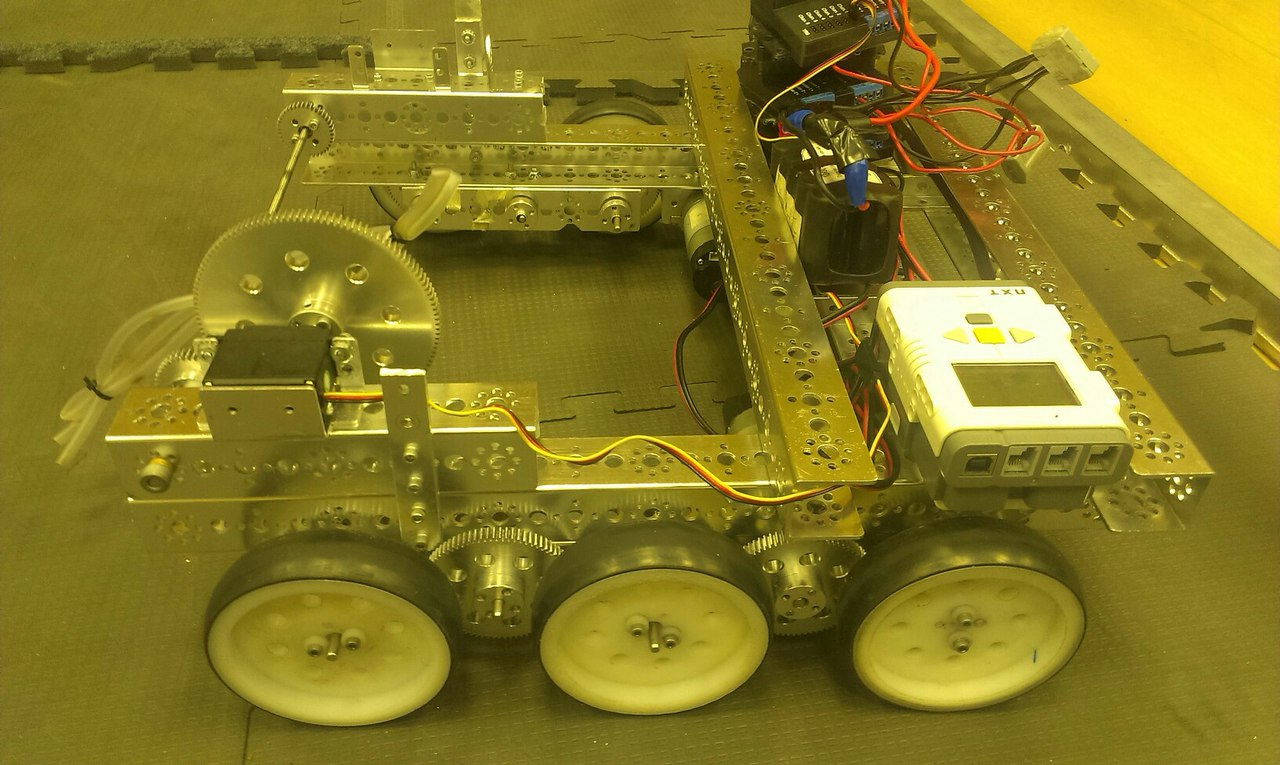
\includegraphics[scale=0.2]{3Engineering/5Team_meetings/days_of_meetings/2015.11.19/images/01}}
		\caption{Wheel base with 10cm wheels}
		\label{Wheelbase1.2}
	\end{minipage}
\end{figure}

